\documentclass{beamer}
\usepackage[utf8]{inputenc}
\usepackage{siunitx}
\usepackage{amsmath}
\usepackage{slashed}
\usepackage{adjustbox}
\usepackage{xcolor}
\hypersetup{
    colorlinks=true,
    linkcolor=blue,
    filecolor=magenta,      
    urlcolor=cyan,
}
\usepackage{hyperref}
\usepackage{multicol}
%#\usepackage{multirow}
\usetheme{boxes}
\newcommand{\Ks}{\ensuremath{K_S^0}}
\newcommand{\ks}{\ensuremath{K_S^0}}
\newcommand{\dd}{\ensuremath{\Delta \delta_D}}
\newcommand{\kspipi}{\ensuremath{\ks \pi^+ \pi^-}}
\newcommand{\Kspipi}{\ensuremath{\ks \pi^+ \pi^-}}
\newcommand{\diffDtokspipi}{\ensuremath{\kspipi{D^0}} \text{and} \ensuremath{\kspipi{\bar{D}^0}} }
\newcommand{\MP}{\ensuremath{m^2_+}}
\newcommand{\MM}{\ensuremath{m^2_-}}
\newcommand{\MZ}{\ensuremath{m^2_0}}
\newcommand{\psires}{\ensuremath{\psi(3770)}}
\newcommand{\phasePosition}{\ensuremath{m^2_+,m^2_-}}
\newcommand{\phasePositionT}{\ensuremath{m^2_-,m^2_+}}
\newcommand{\Dzbar}{\ensuremath{\bar{D}^0} }
\newcommand{\Dz}{\ensuremath{D^0} }
\newcommand{\Bzbar}{\ensuremath{\bar{B}^0} }
\newcommand{\Bz}{\ensuremath{B^0} }
\newcommand{\z}{\ensuremath{\textbf{z}}}
%These macros are save time, usage
%\subAmp{particle}{component} -e.g \subAmp{\Dz}{L_{\pi^+\pi^-}=0}
\newcommand{\subAmp}[2]{\ensuremath{A_{#1}^{#2}\left(\phasePosition \right)}}
%\modelAmp{particle}{model name} - e.g. \modelAmp{\Dz}{Belle}
\newcommand{\modelAmp}[2]{\ensuremath{A_{#1}^{\text{#2}}\left(\phasePosition \right)}}
\newcommand{\genAmp}[2]{\ensuremath{A_{#1}^{\text{#2}}\left(\mathcal{P} \right)}}
%Generic input amp (actually you could use \modelAmp instead if you want
\newcommand{\inputAmp}[1]{\ensuremath{A_{#1}^{\text{input}}\left(\phasePosition\right)}}
%True model - what the decay really is
\newcommand{\trueAmp}[1]{\ensuremath{A_{#1}^{\text{True}}\left(\phasePosition\right)}}
%a_r and phi_r, again saves writing $, _, ^ everywhere
\newcommand{\magPar}[1]{\ensuremath{a_{#1}}}
\newcommand{\phPar}[1]{\ensuremath{\phi_{#1}}}
\newcommand{\KK}{\ensuremath{K^+ K^-}}
\newcommand{\Kppim}{\ensuremath{K^+ \pi^-}}
\newcommand{\Kmpip}{\ensuremath{K^- \pi^+}}
\newcommand{\Kspiz}{\ensuremath{\ks \pi^0}}
\newcommand{\kspiz}{\ensuremath{\ks \pi^0}}
\title{Progress for the Quasi-Model independent method to extract $\dd$ from correlated $D \to \kspipi$ decays}
\begin{document}
\begin{frame}{}
    \maketitle
\end{frame}
%\newcommand{\LLScan}[1]{

\begin{frame}{Likelihood scan for $C_{#1}$}
\includegraphics[width=\textwidth]{2020_04_28/figs/#1_Norm.png}
NB The straight line is a plotting artefact from \texttt{pyplot}
\end{frame}
}


\newcommand{\pull}[2]{
\begin{frame}{Pull distribution for #2 }
\includegraphics[width=\textwidth]{2020_04_28/figs/#1.png}
\end{frame}

}

\newcommand{\pullDist}[3]{
\begin{frame}{Pull distribution for $C_{#1}$ with the #3 tag}
\includegraphics[width=\textwidth]{2020_04_28/figs/pulls/#2_#1.png}
\end{frame}

}
\newcommand{\diffDist}[3]{
\begin{frame}{Pull distribution for $C_{#1}$ with the #3 tag}
\includegraphics[width=\textwidth]{2020_04_28/figs/diffs/#2_#1.png}
\end{frame}

}


\newcommand{\dists}[3]{
\begin{frame}{$C_{#1}$ with the #3}
\begin{columns}
\begin{column}{0.5\textwidth}
\includegraphics[width=\textwidth]{2020_04_28/figs/diffs/#2_#1.png}
\end{column}
\begin{column}{0.5\textwidth}
\includegraphics[width=\textwidth]{2020_04_28/figs/pulls/#2_#1.png}
\end{column}
\end{columns}

Left : Distribution of $C_{#1}^\text{Fit} - C_{#1}^\text{True}$,

right : $(C_{#1}^\text{Fit} - C_{#1}^\text{True})/\sigma C_{#1}^\text{Fit}$
\end{frame}

}

\newcommand{\alldists}[2]{
\dists{00}{#1}{#2}
\dists{01}{#1}{#2}
\dists{10}{#1}{#2}
\dists{02}{#1}{#2}
\dists{11}{#1}{#2}
\dists{02}{#1}{#2}
}

\begin{frame}{Overview}
    \begin{itemize}
        \item After considering physical constraints on $\dd$, we change our proposed ``CP-polynomial'' to an ``anti-symmetric'' polynomial
        \item Widen the range for the likelihood scan for each component
        \item Perform a pull study for the ``anti-symmetric'' polynomial
    \end{itemize}
\end{frame}
\begin{frame}
    Given that 
    \begin{equation}
        \dd(\MM,\MP) = -\dd(\MP,\MM),
    \end{equation}
    and that the model $\dd$ ($\dd^\text{model}$) satisfies this, any correction to $\dd^\text{model}$ ($f(\MM,\MP)$) must also satisfy (1), i.e. the so-called ``CP-Negative'' polynomial, which we will rename to the anti-symmetric polynomial since the function is anti-symmetric along the line $\MM=\MP$, using the parameterisation $w_\pm = (z_+ \pm z_-)/2$ where $z_\pm$ is a re-scaled $m^2_\pm$ such that $z_\pm \in (-1,1)$,
    \begin{equation}
        f(w_-,w_+) = \sum_{i=0}^{N_\text{Order}} \sum_{j=0}^{N_\text{Order} - i} C_{ij} P_{i}(w_+) P_{2j+1}(w_-)
    \end{equation}
\end{frame}

\begin{frame}{$\dd$ plot}
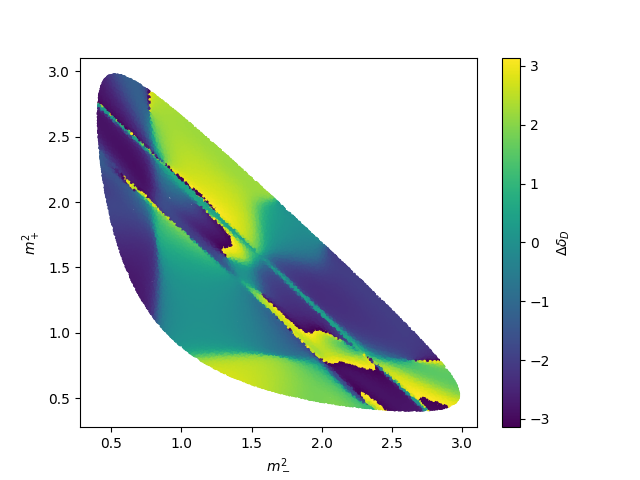
\includegraphics[width=\textwidth]{2020_04_28/figs/dd.png}
\end{frame}
\LLScan{00}
\LLScan{01}
\LLScan{10}
\LLScan{02}
\LLScan{11}
\LLScan{20}

\begin{frame}{Pull Studies}
\begin{enumerate}
    \item Generate $N=10000$ sample from the Belle-BaBar 2018 model
    \item Tags are \KK, \Kspiz, \Kppim, \Kmpip, \Kspipi and the combined tag
    \item \Kppim and \Kmpip tags are modified such that the wrong sign couplings are $-0.0537\pm0.032i$ (back of envelope calculation)
    \item Fit with $N_\text{Order}=2$ polynomial
\end{enumerate}{}
\end{frame}

\pull{KK}{\KK}
\pull{Kmpip}{\Kmpip}
\pull{Kppim}{\Kppim}
\pull{Kspi0}{\Kspiz}
\pull{Kspipi}{\Kspipi}
\pull{Comb}{Combined tags}





\newcommand{\oldpull}[2]{
\begin{frame}{Pull distribution for #2, with constrained coefficients }
\includegraphics[width=\textwidth]{2020_04_28/figs/#1.png}
\end{frame}

}
\newcommand{\pullDist}[3]{
\begin{frame}{Pull distribution for $C_{#1}$ with the #3 tag}
\includegraphics[width=\textwidth]{2020_04_28/figs/pulls/#2_#1.png}
\end{frame}

}
\newcommand{\diffDist}[3]{
\begin{frame}{Pull distribution for $C_{#1}$ with the #3 tag}
\includegraphics[width=\textwidth]{2020_04_28/figs/diffs/#2_#1.png}
\end{frame}

}


\newcommand{\dists}[3]{
\begin{frame}{$C_{#1}$ with the #3}
\begin{columns}
\begin{column}{0.5\textwidth}
\includegraphics[width=\textwidth]{2020_04_28/figs/diffs/#2_#1.png}
\end{column}
\begin{column}{0.5\textwidth}
\includegraphics[width=\textwidth]{2020_04_28/figs/pulls/#2_#1.png}
\end{column}
\end{columns}

Left : Distribution of $C_{#1}^\text{Fit} - C_{#1}^\text{True}$,

right : $(C_{#1}^\text{Fit} - C_{#1}^\text{True})/\sigma C_{#1}^\text{Fit}$
\end{frame}

}

\newcommand{\alldists}[2]{
\dists{00}{#1}{#2}
\dists{01}{#1}{#2}
\dists{10}{#1}{#2}
\dists{02}{#1}{#2}
\dists{11}{#1}{#2}
\dists{02}{#1}{#2}
}

\newcommand{\comparePull}[2]{

\begin{frame}{Comparison of legendre and antisymmetric legendre for the #2 tag}
\begin{columns}
\begin{column}{0.5\textwidth}
\includegraphics[width=\textwidth]{2020_05_06/figs/2/legendre/#1.png}
\end{column}
\begin{column}{0.5\textwidth}
\includegraphics[width=\textwidth]{2020_05_06/figs/2/antiSym/#1.png}
\end{column}
\end{columns}
Left : Pulls for the 2nd order legendre polynomial, right : pulls for the 2nd order antisymmetric polynomial
\end{frame}
}

\begin{frame}{Overview}
We compare the pulls for the two correction functions to $\dd$ for $D \to \kspipi$
\begin{equation*}
\begin{split}
    f_\text{legendre} &= \sum_{i=0}^{N_\text{Order}}\sum_{j=0}^{N_\text{Order} - i} C_{ij}P^\text{legendre}_{i}(z_+)P^\text{legendre}_{j}(z_-) \\ 
    f_\text{antiSym} &= \sum_{i=0}^{N_\text{Order}}\sum_{j=0}^{N_\text{Order} - i} C_{ij}P^\text{legendre}_{i}(w_+)P^\text{legendre}_{2j+1}(w_-) 
\end{split}
   
\end{equation*}
where 
\begin{equation*}
    \begin{split}
       z_\pm &= \frac{m_\pm^2 - (\max m_\pm^2 + \min m_\pm^2)}{\max m_\pm^2 - \min m_\pm^2} \\
       w_\pm &= \frac{1}{2} \left(z_+ \pm z_- \right)
    \end{split}
\end{equation*}
\end{frame}

\begin{frame}{Overview 2}
\begin{enumerate}
    \item $C_{ij}$ was originally constrained to $|C_{ij}| < \frac{2 \pi}{(N_\text{Order} + 1)(N_\text{Order + 2})}$, but this kills off higher order polynomials since $P^\text{legendre}_{i+1}(x) << P^\text{legendre}_i(x)$.
    \item ``Combined'' Log likelihood does indeed produce the sum of all likelihoods per tag
    \end{enumerate}
\end{frame}

\comparePull{Comb}{Combined}
\oldpull{Comb}{Combined}
\comparePull{KK}{$\KK$}
\oldpull{KK}{$\KK$}
\comparePull{Kppim}{$\Kppim$}
\oldpull{Kppim}{$\Kppim$}
\comparePull{Kmpip}{$\Kmpip$}
\oldpull{Kmpip}{$\Kmpip$}
\comparePull{Kspi0}{$\Kspiz$}
\oldpull{Kspi0}{$\Kspiz$}
\comparePull{Kspipi}{$\Kspipi$}
\oldpull{Kspipi}{$\Kspipi$}

\end{document}